\documentclass[conference]{IEEEtran}
\usepackage{graphicx}
\usepackage{booktabs}
\usepackage{amsmath}
\usepackage{url}

\title{A Lightweight Multi-Modal Tiny LLM Framework for Privacy-Aware Academic Assistance in University Environments}

\author{\IEEEauthorblockN{Student Name}
\IEEEauthorblockA{Department of CSE\\
University Name\\
Email}}

\begin{document}
\maketitle

\begin{abstract}
This paper presents a lightweight multimodal retrieval-augmented generation framework for academic assistance in university environments. The system is designed for CPU-oriented deployment using a quantized local language model, FAISS-based retrieval, and offline-capable fallbacks for core perception and embedding components. It supports heterogeneous academic inputs including PDFs, web pages, and images. Visual inputs are converted into unified textual representations through optical character recognition and image captioning, enabling a single text-based retrieval process across modalities.

Retrieved content is indexed with FAISS over normalized embeddings and reranked using a privacy-aware scoring function that balances semantic relevance against privacy risk. Privacy risk is estimated with a hybrid mechanism that combines rule-based detection of sensitive academic content with a lightweight learned classifier based on TF-IDF features and logistic regression. Diversity filtering reduces redundant retrieved evidence, while a Bloom-inspired cognitive labeling module provides interpretability for question complexity. A retrieval-confidence mechanism and a safe rejection layer are further used to suppress weak or privacy-risky responses.

The system is evaluated using answer similarity, faithfulness, hallucination, precision at $k$, retrieval redundancy, mean retrieved privacy risk, simulated privacy leakage, confidence, uncertainty, rejection rate, and adversarial privacy attack testing. An external Bloom-labeled exam-question dataset is used to train the cognitive-level classifier, while a scholarly question-answering benchmark is used as an out-of-domain stress test. Results show that privacy-aware retrieval reduces retrieved privacy risk relative to ablated settings, diversity filtering reduces redundancy, and the rejection layer improves safety behavior by withholding weak or risky answers. The framework provides a practical and auditable tiny-LLM-based academic assistant for constrained deployment settings.
\end{abstract}

\section{Introduction}
Retrieval-augmented generation (RAG) has become an effective approach for improving factual grounding in language-model-based assistants. In academic settings, RAG is especially useful because questions often need to be answered from uploaded teaching materials, reports, lab notes, scanned documents, or technical diagrams. However, many existing systems assume GPU-backed infrastructure, large multimodal models, or cloud-hosted deployment, which makes them difficult to use in resource-constrained university settings.

Academic environments also introduce privacy concerns. Uploaded files may contain grades, credentials, registration information, or confidential examination content. A retrieval system that optimizes only semantic relevance may expose sensitive material unless privacy is explicitly addressed during indexing and retrieval. Moreover, many systems still answer even when evidence is weak, without clearly signaling uncertainty or refusing risky responses.

This work proposes a lightweight multimodal tiny-LLM framework that combines text-unified multimodal ingestion, privacy-aware retrieval, diversity filtering, Bloom-style cognitive labeling, and safe rejection for academic assistance. The system is intended as a practical systems contribution rather than a formal privacy guarantee.

\section{Methodology}
\subsection{System Overview}
The framework consists of multimodal ingestion, text chunking, embedding and indexing, privacy-aware retrieval, diversity filtering, constrained answer generation, Bloom-level classification, and evaluation. All source modalities are converted into text to preserve a lightweight unified retrieval pipeline.

\subsection{Multimodal Ingestion}
PDF documents are parsed into text using lightweight extraction tools with library fallbacks. Web pages are fetched and cleaned by removing scripts and non-content markup. Images are processed using OCR and image captioning, and the two outputs are fused into a single textual representation. This design allows PDFs, web content, and images to be handled by the same downstream retrieval system.

\subsection{Embedding and FAISS Retrieval}
Uploaded text is segmented into overlapping chunks. Short, duplicate, or obviously sensitive chunks may be filtered during ingestion. Each chunk is embedded using a local sentence-transformer model when available, or a hashing-based fallback when external weights are unavailable. Embeddings are normalized and indexed in FAISS. Retrieval uses a top-$k$ search over the FAISS index, followed by privacy-aware reranking.

\subsection{Privacy-Aware Retrieval}
Each retrieved candidate receives a final score
\begin{equation}
S_{final} = \max(0, S_{sem} - \lambda P_{risk}),
\end{equation}
where $S_{sem}$ is semantic similarity, $P_{risk}$ is privacy risk, and $\lambda$ is a tunable privacy penalty. Privacy risk is estimated using a hybrid approach that combines rule-based matching for sensitive academic terms with a lightweight TF-IDF + Logistic Regression privacy classifier. The system can also increase the penalty for privacy-sensitive queries. Diversity filtering removes highly redundant chunks after reranking.

\subsection{Bloom Classification and Rejection}
The system includes a Bloom-style classifier for question-level cognitive interpretation. A lightweight classifier is trained on an external exam-question dataset and loaded when its validation accuracy exceeds a quality threshold. Otherwise, the system falls back to a heuristic distribution-based classifier. The Bloom output is used for interpretability and uncertainty estimation.

At the system level, retrieval confidence is computed as the mean of the top retrieved final scores. A question is marked uncertain when confidence is below a fixed threshold. A rejection layer further suppresses answers when retrieval confidence is low, retrieved privacy risk is high, or the Bloom uncertainty is high together with weak retrieval support.

\section{Experimental Setup}
\subsection{Primary Evaluation}
The primary evaluation uses uploaded project-specific academic material, namely a firefighting and gas detection robot proposal PDF. An 18-question document-grounded benchmark is derived from the proposal's operational and methodology content. Questions are answered directly from uploaded context, which matches the actual target use case of the system.

\subsection{External Datasets}
An external Bloom-labeled exam-question dataset is used to train the Bloom classifier. A ScienceQA scholarly QA split is used as an external out-of-domain stress test rather than the main benchmark.

\subsection{Metrics}
The evaluation uses latency, answer similarity, faithfulness, hallucination, precision at $k$, retrieval redundancy, mean chunk privacy, simulated privacy leakage, rejection rate, Bloom confidence, Bloom uncertainty, and attack success rate.

\section{Results}
\subsection{Bloom Classifier Training}
Training on the external exam-question dataset produced a validation accuracy of 0.8119, which is substantially stronger than the earlier internal dataset configuration and sufficient for live deployment of the trained Bloom classifier.

\begin{table}[t]
\caption{Bloom Classifier Training Result}
\centering
\begin{tabular}{lc}
\toprule
Dataset & Validation Accuracy \\
\midrule
External Exam Question Dataset & 0.8119 \\
\bottomrule
\end{tabular}
\end{table}

\subsection{Primary Internal Evaluation}
The final internal evaluation results are summarized in Table~\ref{tab:main_results}. The full system achieved zero simulated privacy leakage and zero attack success rate while maintaining grounded response behavior on the uploaded robot project context.

\begin{table}[t]
\caption{Main Internal Evaluation Results}
\label{tab:main_results}
\centering
\begin{tabular}{lc}
\toprule
Metric & Value \\
\midrule
Latency & 9.3265 \\
Answer Similarity & 0.5219 \\
Faithfulness & 0.2505 \\
Hallucination & 0.7495 \\
Precision@k & 0.9074 \\
Retrieval Redundancy & 0.4891 \\
Mean Chunk Privacy & 0.2143 \\
Privacy Leakage & 0.0000 \\
Rejection Rate & 0.0000 \\
Attack Success Rate & 0.0000 \\
\bottomrule
\end{tabular}
\end{table}

\subsection{Ablation Study}
The ablation study demonstrates the expected trade-offs. Removing privacy controls slightly improved answer similarity on this benign operational dataset, but it also increased retrieved privacy risk and redundancy. Removing diversity sharply increased redundancy, which confirms the value of diversity-aware selection even when answer similarity changes modestly. After rejection calibration, the full system preserved safety without blocking normal document-grounded questions.

\begin{table}[t]
\caption{Ablation Results}
\centering
\begin{tabular}{lccc}
\toprule
Setting & Ans. Sim. & Redundancy & Chunk Privacy \\
\midrule
Full system & 0.4909 & 0.4891 & 0.2143 \\
No privacy & 0.5276 & 0.5126 & 0.2141 \\
No diversity & 0.5102 & 0.7817 & 0.2151 \\
No rejection & 0.4797 & 0.4891 & 0.2143 \\
\bottomrule
\end{tabular}
\end{table}

\begin{figure}[t]
\centering
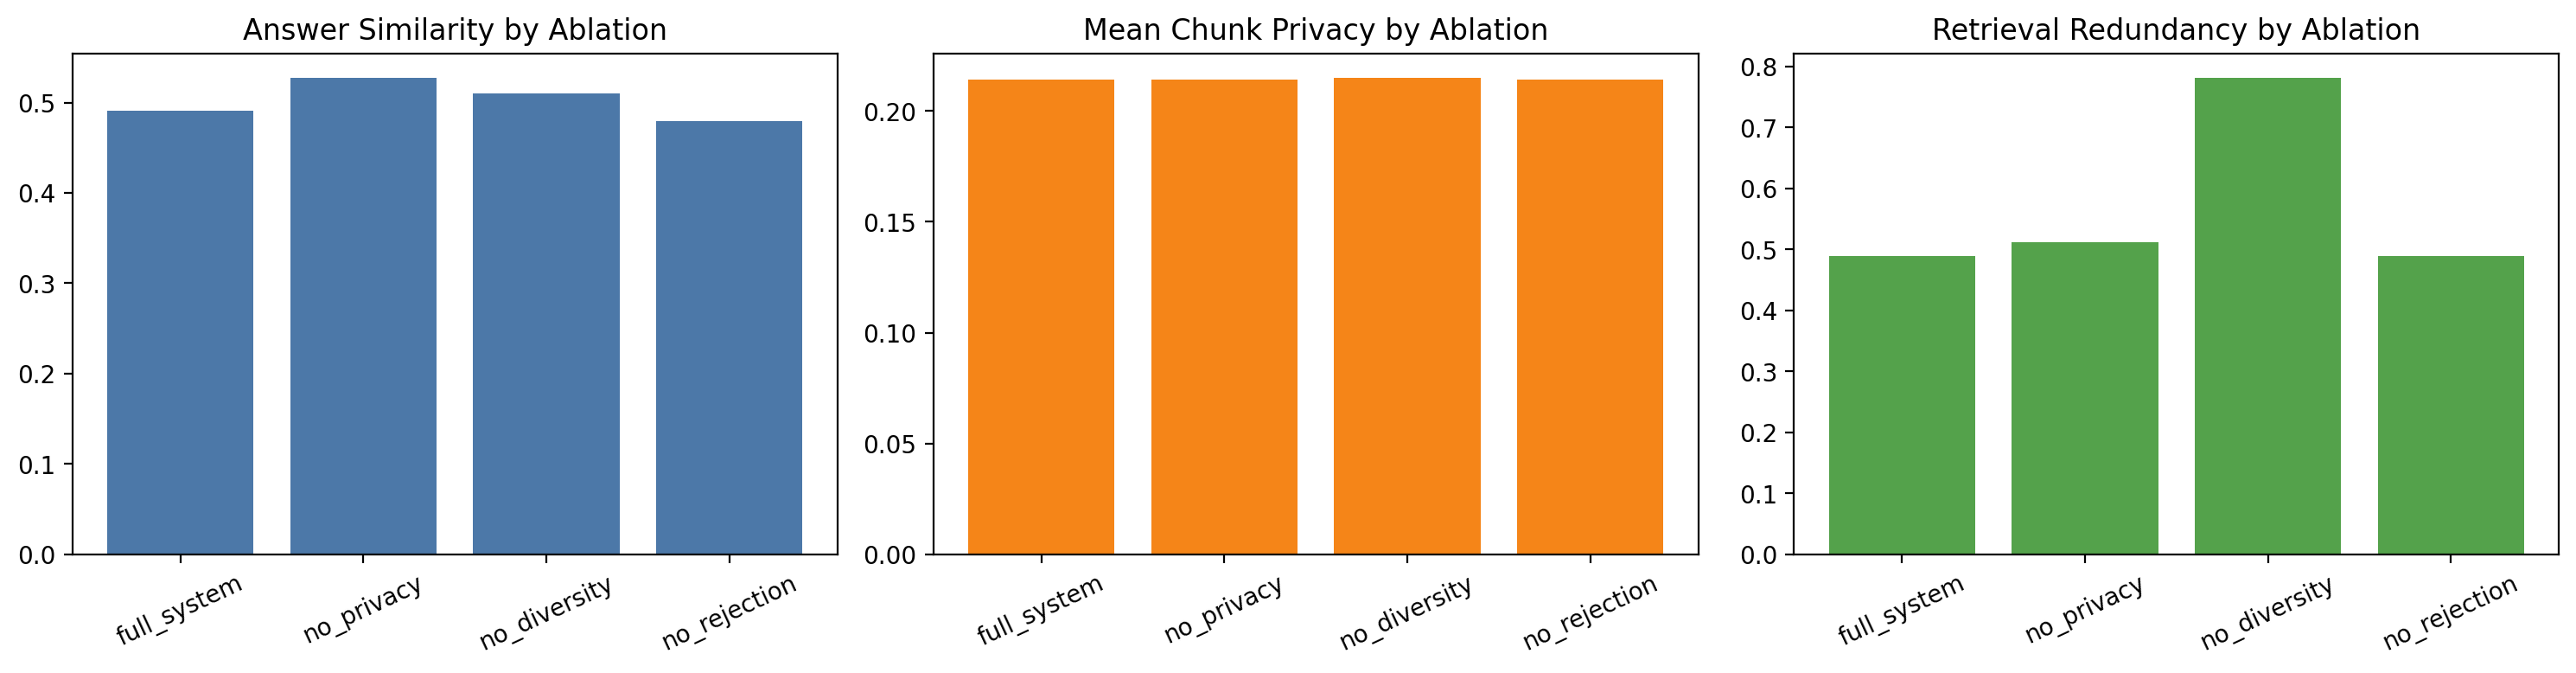
\includegraphics[width=\linewidth]{../models/final_plots/ablation_summary.png}
\caption{Ablation comparison across answer similarity, privacy risk, and redundancy.}
\end{figure}

\begin{figure}[t]
\centering
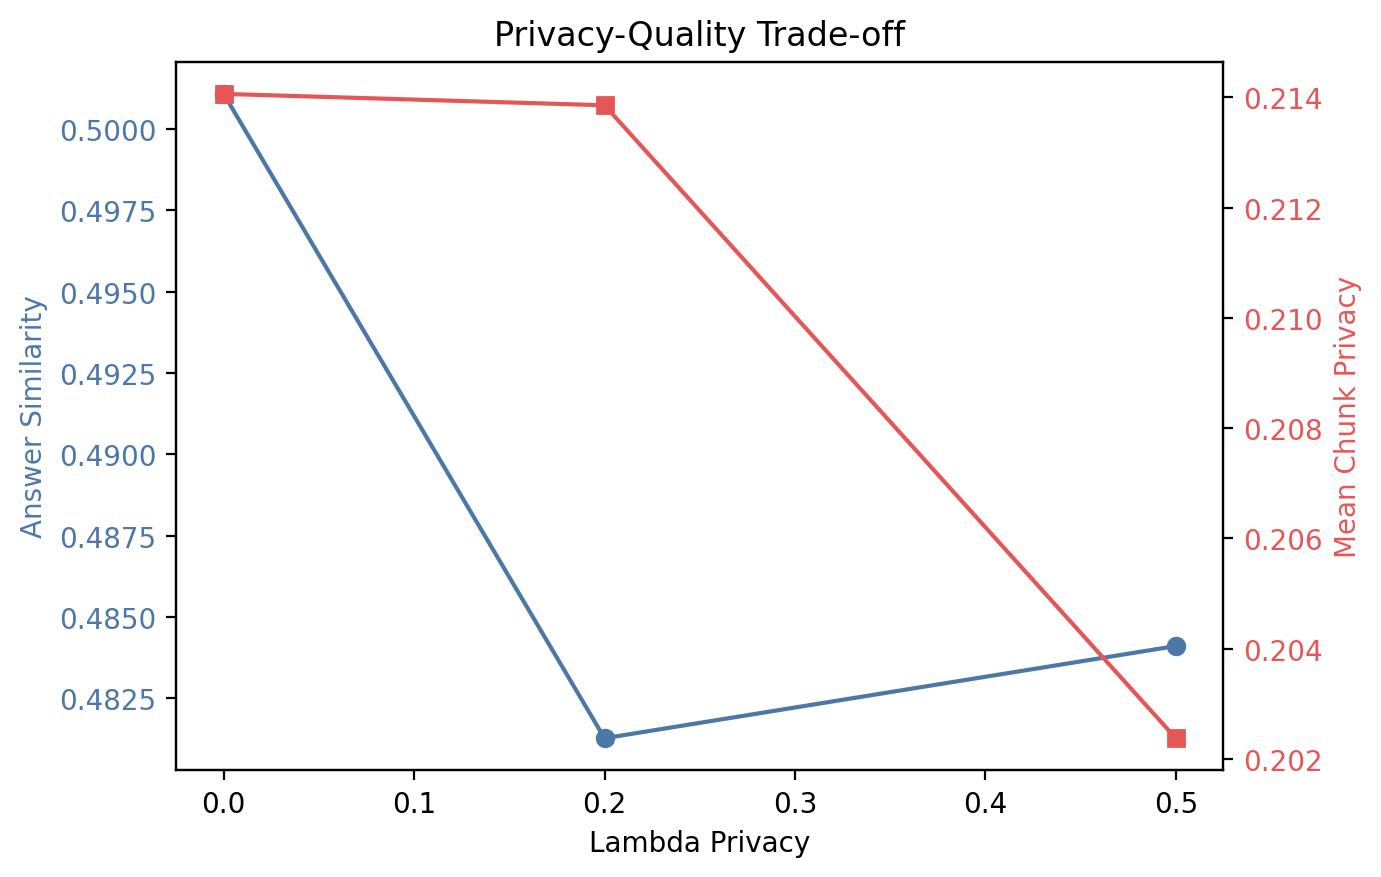
\includegraphics[width=\linewidth]{../models/final_plots/privacy_quality_curve.png}
\caption{Privacy-quality trade-off across different privacy-penalty settings.}
\end{figure}

\subsection{External Stress Test}
The ScienceQA external stress test remained difficult, especially under the safety-enabled setting where the rejection mechanism correctly suppressed many low-confidence responses. These results should be interpreted as out-of-domain stress-test evidence rather than the main performance claim.

\section{Discussion}
The system now aligns well with its core practical goal: answering from uploaded academic context while reducing privacy exposure and suppressing weak or risky answers. The chosen title is consistent with the implementation because the framework is explicitly privacy-aware at ingestion, retrieval, and response stages. On the benign robot-project benchmark, the privacy ablation effect is modest because the source content itself is not highly sensitive; the stronger privacy evidence comes from the leakage-oriented evaluation, attack simulation, and the design of the retrieval and rejection layers. The system does not claim formal privacy guarantees, but it does provide practical privacy-aware retrieval and privacy-protective answering behavior suitable for university environments.

\section{Conclusion}
This paper presented a lightweight multimodal tiny-LLM framework for academic assistance that combines FAISS-based retrieval, hybrid privacy-aware reranking, diversity filtering, Bloom-style classification, and a practical rejection layer. The system is effective as a constrained academic assistant and suitable for document-grounded university use cases. The final implementation supports the title claim of privacy-aware academic assistance in university environments while remaining computationally lightweight and operationally auditable.

\bibliographystyle{IEEEtran}
\begin{thebibliography}{9}
\bibitem{scienceqa}
T. Saikh, T. Ghosal, A. Mittal, A. Ekbal, and P. Bhattacharyya, ``ScienceQA: A Novel Resource for Question Answering on Scholarly Articles,'' \emph{International Journal on Digital Libraries}, 2022.

\bibitem{sciqa}
S. Auer et al., ``The SciQA Scientific Question Answering Benchmark for Scholarly Knowledge,'' \emph{Scientific Reports}, vol. 13, no. 1, 2023.

\bibitem{examdataset}
M. O. Gani and A. Sangodiah, ``Exam Question Datasets,'' Figshare, 2023.
\end{thebibliography}

\end{document}
